Fin dagli albori di Internet alcuni agenti commerciali intuirono il potenziale offerto dalla vendita on-line e cominciarono a presidiare il nuovo canale di vendita dando vita al commercio elettronico, o e-commerce.
\newline
Storicamente il termine e-commerce ha visto mutare il proprio significato: nel 1970, il termine “e-commerce” si riferiva a scambio elettronico di dati per l’invio dei documenti aziendali come gli ordini di acquisto. Successivamente, grazie allo sviluppo tecnologico, il commercio elettronico è diventato un’attività di scambio di beni e servizi attraverso il Web \cite{commerce_intro_1}, permettendo di consolidare l’abitudine ad acquistare on-line da parte dei clienti, che hanno, così aumentato la quota di spesa on-line sul consumo totale.
\newline
Il cambio radicale che internet sta apportando nella società investe consistentemente anche le abitudini di acquisto dei consumatori che dimostrano sempre più fiducia nel mezzo elettronico, preferendo sempre più frequentemente l’acquisto on-line rispetto all’acquisto in negozio.
\newline
I principali vantaggi che ha apportato questa nuova modalità di acquisto sono comodità, accessibilità e vantaggio economico.
\newline
Per comodità si intende il fatto che sia posibile scegliere, ordinare ed acquistare il bene desiderato direttamente da casa senza la necessità di recarsi in un negozio fisico.
\newline
L'accessibilità è il fattore che permette al consumatore di accedere agli store on-line h24, consentendo un confronto tra prodotti offerti a livello internazionale.
\newline
Il vantaggio economico è uno dei punti salienti nonchè il piu convincente, in quanto gli store on-line riescono a garantire prezzi più bassi in virtù delle minori spese che devono sostenere.
\begin{figure}[htb]
 \centering
 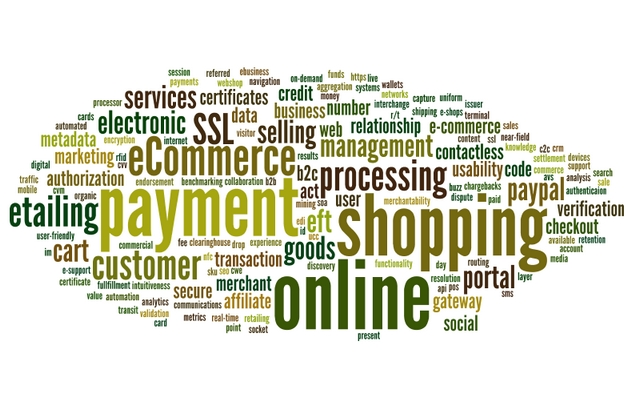
\includegraphics[width=0.8\linewidth]{images/introduction/ecommerce-wordle.jpg}\hfill
 \caption[e-commerce wordle]{e-commerce wordle}
 \label{fig:e_commerce_wordle}
\end{figure}
\newline
La forte competizione e la velocità che caratterizzano il mercato on-line accentuano l’importanza del “time to market”, ovvero la rapidità con cui una azienda riesce ad arrivare al dispiegamento di tutti gli apparati necessari a raggiungere il cliente.
\newline
E' dunque il Web, il primo canale per le aziende che permette loro di affermarsi sul mercato e aumentare il proprio profitto.
Tale processo, innanzitutto, inizia con la creazione di un proprio sito istituzionale, un vero e proprio “biglietto da visita”, per mostrarsi al mondo digitale.
\newline
Per semplificare e velocizzare il processo di creazione e messa in produzione di ambienti di e-commerce sono apparsi nel tempo numerosi servizi.
\newline
Shopify, Bigcommerce, Prestashop, 3dcart, WIX.com sono alcune tra le piattaforme più note ed utilizzate, che offrono la possibilità di inserire, modificare e cancellare prodotti, gestire l’inventario, creare collezione di prodotti, mettendo a disposizione uno o più servizi di pagamento, spedizione/tracking, etc.. Il tutto attraverso un’interfaccia di facile utilizzo in maniera tale che, chiunque possa usufruirne.
\newline
In generale tali prodotti sono ben consolidati quindi affidabili. Di contro però, per via del fatto che esistono da diversi anni, risultato sviluppati con tecnologie per cui ad oggi esistono moderni e validi sostituti.
\newline
Il lavoro presentato in questa tesi, svolto presso il CVDLAB, è consistito nello studio ad alto livello delle principali piattaforme di e-commerce oggi esistenti, al fine di individuare un modello dei dati astratto capace di sintetizzare le caratteristiche di valore offerte.
Ottenuto il modello è stata implementata una nuova piattaforma, X-commerce, sfruttando
tecnologie moderne come Polymer, Loopback e Nodejs.
\newline
X-commerce utilizza pervasivamente Polymer, che implementa lo standard dei Web Components \cite{web_comt_std}, la cui caratteristica principali è la riusabilità del codice.
Come detto dagli autori di Polymer-Project: “Tutto è un elemento” \cite{polymer_world_view}. Questa è la filosofia che X-commerce segue, per cui ogni tipo di funzione o responsabilità è incapsulata in elementi Polymer diversi ed auto-contenuti.
Dunque X-commerce ha come obiettivo  quello di estremizzare il concetto di Web Components fino alla realizzazione di una piattaforma di larga scala, e-commerce.
\newline
X-commerce mira ad offrire agli sviluppatori un nuovo metodo, basato su componenti riutilizzabili, per comporre le proprie pagine web (orientati all’e-commerce). Quindi, la realizzazione di una pagina web avviene componendo i diversi elementi.
\newline
La tesi si articola in due parti: la prima tratta della storia dell'arte, dei servizi indispensabili per i sistemi di e-commerce e delle tecnologie utilizzate, mentre la seconda affronta in dettaglio la descrizione del progetto x-commerce nella sua interezza.
In particolare il primo capitolo illustra lo stato dell’arte sulle piattaforme che facilitano la realizzazione di sistemi e-commerce come Shopify, Bigcommerce, Prestashop, etc.
Il secondo capitolo descrive le i principali provider abilitanti per i servizi di pagamento ed il terzo mostra una panoramica generale sulle principali tecnologie utilizzate per realizzare X-commerce come Polymer, Loopback, etc.
\newline
Nel quarto capitolo viene descritta l'architettura di X-commerce evidenziando i principali schemi e modelli dello stesso.
\newline
Il quinto si focalizza principalmente sulla gestione dei pagamenti, servizio indispensabile per un sistema di e-commerce mentre il sesto ed ultimo espone le conclusioni tratte e fornisce dei possibili sviluppi futuri per il progetto.
